%compile with writelatex.com
\documentclass[a4paper]{article}
\usepackage[english]{babel}
\usepackage[utf8]{inputenc}
\usepackage{amsmath}
\usepackage{graphicx}
\usepackage{pgfplots}%plotting graphs
\usepackage{epigraph}%for quotes
%\epigraphfontsize{\small\itshape}
\setlength\epigraphwidth{1\textwidth}
\setlength\epigraphrule{0pt}
\usepackage[colorinlistoftodos]{todonotes}
\usepackage{color}
\usepackage{hyperref}
\usepackage{float}
\usepackage{fancyhdr}
\usepackage{sidecap}%enables figcap next to picture for larger captions
\usepackage[yyyymmdd,hhmmss]{datetime}%for generating auto time stemp
%from geogebra
\usepackage{pstricks-add}
\usepackage{pgf,tikz}
\usetikzlibrary{arrows}
\newrgbcolor{xdxdff}{0.49 0.49 1}
\newrgbcolor{uququq}{0.25 0.25 0.25}
\newrgbcolor{vvvvvv}{0.33 0.33 0.33}
\newrgbcolor{ayayay}{0.66 0.66 0.66}
\newrgbcolor{srsrsr}{0.13 0.13 0.13}
\definecolor{qqwuqq}{rgb}{0.13,0.13,0.13}
\definecolor{uququq}{rgb}{0.25,0.25,0.25}
\definecolor{xdxdff}{rgb}{0.66,0.66,0.66}
\definecolor{qqqqff}{rgb}{0.33,0.33,0.33}
\newcommand{\degre}{\ensuremath{^\circ}}
\psset{xunit=1.0cm,yunit=1.0cm,algebraic=true,dotstyle=o,dotsize=3pt 0,linewidth=0.8pt,arrowsize=3pt 2,arrowinset=0.25}
%end from geogebra
\renewcommand{\deg}{\ensuremath{^{\circ}}}%enable degree symbol for angles and celcius
\pagestyle{fancy}
\newcommand{é}{\'e}
\newcommand{ë}{\"e}
%edit this if you need a different date
\newcommand{\todayDate}{\today}
\rfoot{Compiled on \todayDate\ at \currenttime GMT}
\cfoot{}
\lfoot{Page \thepage}


\begin{document}
    \centering

	\title{Les 01\\*
		\small
		$\in$\\*
		homework assignments\\*
		$\subset$\\*
		Continue wiskunde en statistiek}
	\author{\href{http://svlentink.co.nf}{Sander Lentink} \small 10422439 \\*
		\small
        	Artificial intelligence,
            \href{http://uva.nl}{Universiteit van Amsterdam},
            the Netherlands}

	\date{\todayDate}

\maketitle

\scriptsize - The pdf version of this document contains hyperlinks. -
\normalsize

\section{2.3.19}
A function $y = f(x)$ with a vertical asymptote at $x = 1$ and a slanting asymptote $y = x + 1$
when $x \to \pm \infty$.

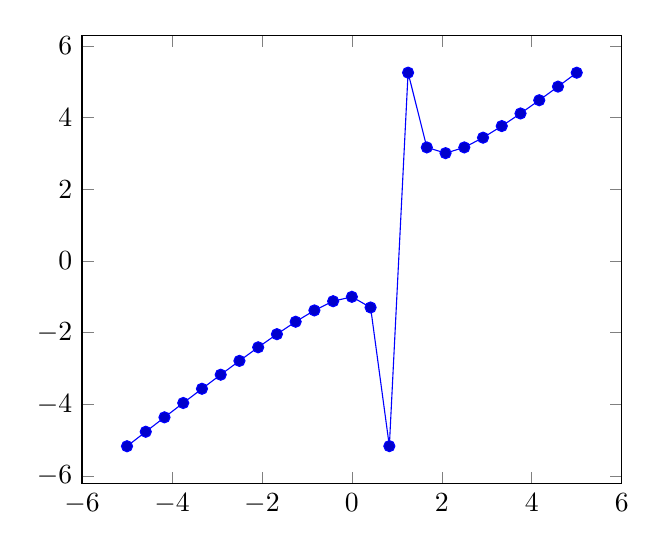
\begin{tikzpicture}
  \begin{axis}[ 
    %xlabel=$x$,
    %ylabel={$y$}
  ] 
    \addplot {x+ (1)/(x-1)}; 
  \end{axis}
\end{tikzpicture}

\begin{equation}
f(x) = x + \frac{1}{x-1}
\end{equation}

\newpage

\section{2.3.21}

\begin{equation}
\href{http://www.wolframalpha.com/input/?i=lim+x+to+infinity%2C+x%5E2%2F%28x-1%29+-+x}{\lim_{x \to \infty} \frac{x^2}{x-1} - x}
\Rightarrow
\lim_{x \to \infty} \frac{x}{x-1}
\href{http://www.wolframalpha.com/input/?i=lim+x+to+infinity%2C+x%2F%28x-1%29}{= 1}
\end{equation}

\section{2.3.23}

\begin{equation}
\href{http://www.wolframalpha.com/input/?i=lim+x+to+infinity%2C+x%5E2%2F%28x-1%29+-+x}{ \lim_{x \to \infty} x \ln(1 + \frac{1}{x}) }
\Leftrightarrow
\lim_{x \to \infty} \ln( (1 + \frac{1}{x})^x )
= 1
\end{equation}

$\lim_{x \to \infty} (1 + \frac{1}{x})^x$ gives us the Euler constant \textit{e}. And $\log_a(a) = 1$.

\section{5.8.13}

\begin{equation}
\href{http://www.wolframalpha.com/input/?i=%7Cx%5E2+%2B+3x+%2B+2%7C}{h(x) = |x^2 + 3x + 2|}
\Leftrightarrow
|(1+x)(x+2)|
\end{equation}


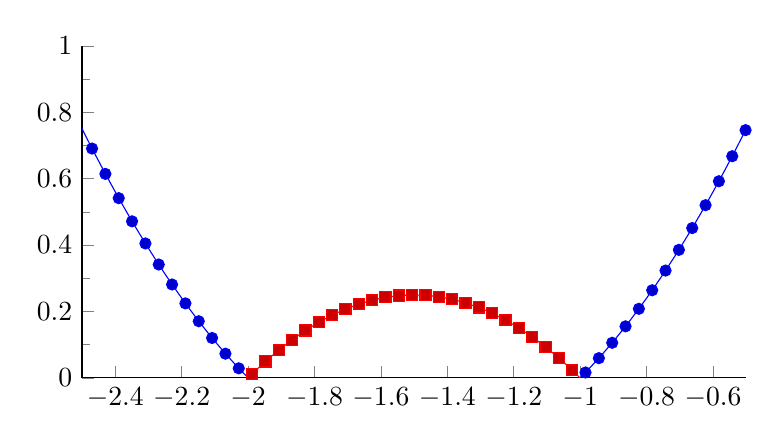
\begin{tikzpicture}
  \begin{axis}[
  samples=250,
  unbounded coords=jump,
  scale only axis,
  xmin=-2.5, xmax=-.5,
  ymin=0, ymax=1,
  axis lines*=left,
  axis equal image,
  minor y tick num=1
    %xlabel=$x$,
    %ylabel={$y$}
  ] 
    \addplot {(x*x + 3*x + 2)};
    \addplot {-1*(x*x + 3*x + 2)}; 
  \end{axis}
\end{tikzpicture}


We find the points $-2$ and $-1$ to be \textbf{non-differentiable}.


\section{5.8.15}

Using the derivatives table,
\href{http://www.wolframalpha.com/input/?i=sin%28x%5E2%29}{$f(x) = \sin(x^2)$}
gives us
\href{http://www.wolframalpha.com/input/?i=2x+cos%28x%5E2%29}{$f(x)' = 2 x \cos(x^2)$},
from which we get to
$f(x)'' = 2 \cos(x^2) - 4 x^2 \sin(x^2)$.


\end{document}
